\section{Topic Tree}
\subsection{Overview}
Most learning management systems do not have a simple and easy method to import course material and resources from other courses. Some LMS platforms such as OpenLearning have no method of importing any data at all, and other platforms such as Canvas allows you to import crowd sourced material into your own course, however still does not allow you to import topics of resources. \\

This new LMS has a new topic tree feature, which will allow teachers and academics to add course material under a specific topic instead.\\

\textbf{Topics} \\
A topic is a collection of educational material that is related to a particular subject. For example, in UNSW's Introduction to Programming course (COMP1511), one of the topics in the course is ``Pointers", which contains all course material related to pointers.\\

At Charles Sturt University, each topic is defined as a small subject that is three hours in length \cite{csutopictree}. CSU's curriculum covers around 1000 topics with each topic being three hours in length for a degree. In this thesis, we will also define a topic being three hours of content, but instructors can choose what amount of content constitutes as a topic.\\

\textbf{Topic Groups} \\
Topic groups are similar to courses themselves, except they are purely for organisational and enrolment purposes. We found that it would be much easier to enrol students into a group of topics instead of each individual topic, and it makes searching the topic tree much easier as there are a smaller number of topic groups than topics themselves. \\

Topic groups themselves do not contain assessments, exams, or any other resources. Only topics themselves contain this information. Therefore, academics must store assessments in individual topics and set up the prerequisites so if they wish, they can store a final exam in the last topic that students must complete or in an empty "milestone" topic. We decided to name this grouping of topics as "topic groups" instead of courses due to how a traditional course contains assessments and other content for the entire course, and does not have prerequisites between the topics themselves. This naming helps differentiate the system from the traditional university model.\\

\textbf{Prerequisites} \\

Each topic can have its own prerequisites, as discussed briefly previously. Some topics must be completed in order to complete the current topic. Prerequisites can be across topic groups as well. For example, Linked Lists in the "Introduction to Programming" topic group must be completed in order to start Graphs in "Data Structures and Algorithms". This improves reusability, as topics in other topic groups can be set as prerequisites eg. Git can be set a prerequisite for "Web Front end Programming" instead.

\textbf{Reusability} \\
The topic tree enables academics to easily reuse content - by setting specific topics, academics can reuse content instead of creating new content for the same topic in their own course. A good example of this is "Web Front end Programming" at UNSW - Instead of creating new content for Git, academics can set Git as a prerequisite. However, to encourage reusability, a cloning feature is also provided where academics can clone a topic and its resources from another topic group and put it in its own topic group. This further enables reusability, demonstrating that there is no need to spend time creating new content.\\

\textbf{Course Materials} \\
The Meta Learning Management System also organises content into four sections:
\begin{itemize}
    \item Content
    \item Practice
    \item Preparation
    \item Assessments
\end{itemize}

These various sections were chosen as they fit many learning models, including UNSW's learning models as listed on their website \cite{learningModel}. Students are introduced to it in the content section, and then get to know more about it in the practice section, and try it out in the preparation and assessments sections. After receiving feedback, this cycle repeats again.\\

\begin{figure}[h!]
    \centering
    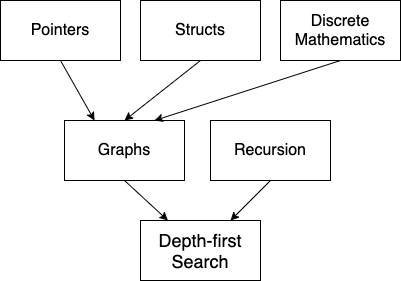
\includegraphics[scale=0.4]{topic-tree-example}
    \caption{Example of a topic tree with Depth first search}
\end{figure}

In the above example, pointers, structs and discrete mathematics must be learned in order to learn graphs. Likewise, graphs and recursion is required to learn depth first search.\\

\subsection{Requirements}
Each requirement will have a priority: High, Medium or Low. High priority requirements will be completed first, and then medium and low priority requirements respectively. \\

\subsection{Functional Requirements}

\textbf{Viewing Topics}

\begin{table}[]
\begin{tabular}{ll}
\textit{As a}      & User                                                \\
\textit{I want to} & View groups of topics                               \\
\textit{So that}   & I can see how topic groups interact with each other
\end{tabular}
\end{table}

\begin{table}[]
\begin{tabular}{ll}
As a      & User                                                \\
I want to & View topics within each group                       \\
So that   & I can see how topic groups interact with each other
\end{tabular}
\end{table}

    \begin{enumerate}
    \item Users can view groups of topics \textcolor{Orange}{Medium}
    \item Users can view topics within each group \textcolor{Red}{High}
    \item Users can search for a topic \textcolor{Red}{High}
    \item Users can search for specific resources \textcolor{Red}{High}
    \item Users can view topic prerequisites \textcolor{Orange}{Medium}
    \item Users can view a graph of topics and their prerequisites \textcolor{Red}{High}
    \item Users can view the topic tree with a traditional interface \textcolor{Blue}{Low}
    \end{enumerate}

\textbf{Adding Topics and resources}
    \begin{enumerate}
    \item Users can add a new topic \textcolor{Red}{High}
    \item Users can upload course material \textcolor{Red}{High}
    \item Users can add a new topic group \textcolor{Orange}{Medium}
    \end{enumerate}

\textbf{Deleting Topics}
    \begin{enumerate}
    \item Users can delete a topic that they've created \textcolor{Red}{High}
    \item Users can delete a topic group that they've created \textcolor{Orange}{Medium}
    \item Users can remove course material from a topic \textcolor{Red}{High}
    \end{enumerate}

\textbf{Topic Prequisites}
    \begin{enumerate}
    \item Users can add a topic prerequisite \textcolor{Orange}{Medium}
    \item Users can delete a topic prerequisite \textcolor{Orange}{Medium}
    \end{enumerate}

\textbf{Integration}
    \begin{enumerate}
    \item Users can import course material by selecting topics for a course \textcolor{Red}{High}
    \item Users can remove topics from a course \textcolor{Red}{High}
    \end{enumerate}

\textbf{Exporting}
    \begin{enumerate}
    \item Users can export data from topics and course material \textcolor{Blue}{Low}
    \end{enumerate}

\subsection{Timeline}
This timeline details what is planned over the course of the year to achieve a working topic tree feature in the meta learning management system.
Milestones are featured throughout this timeline.

\newpage

\begin{figure}[h!]
    \centering
    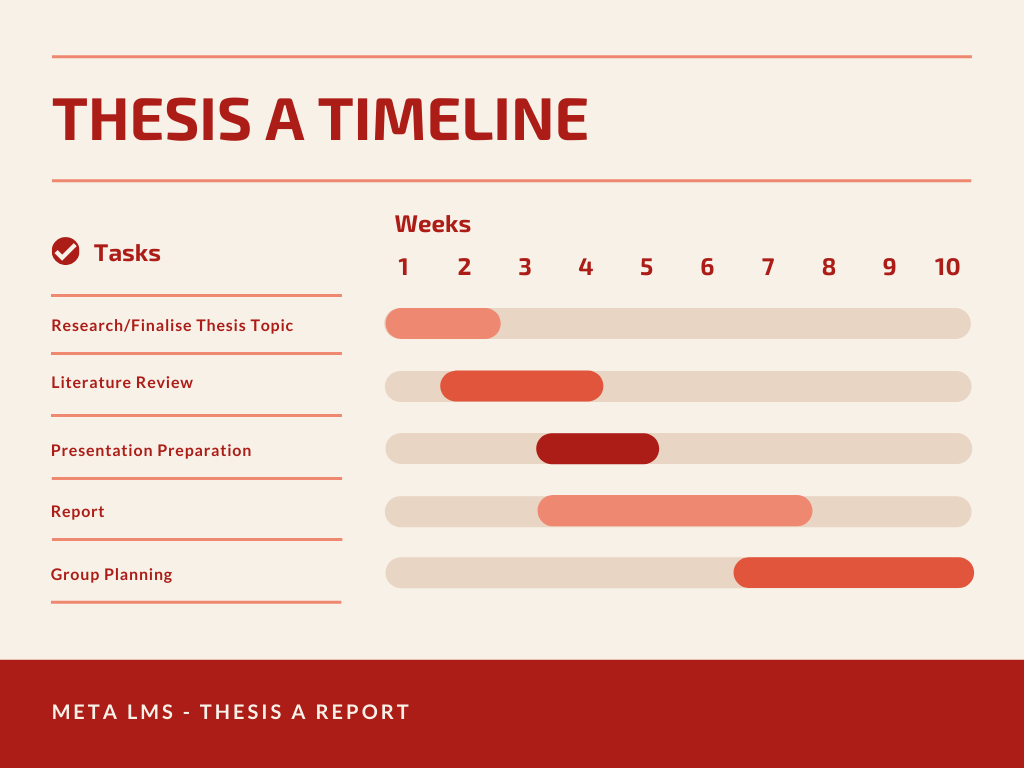
\includegraphics[scale=0.4]{topic-tree-thesis-a}
    \caption{Thesis A Timeline}
\end{figure}

This term, the focus is literature review and planning features for implementation in Thesis B and C.


\begin{figure}[h!]
    \centering
    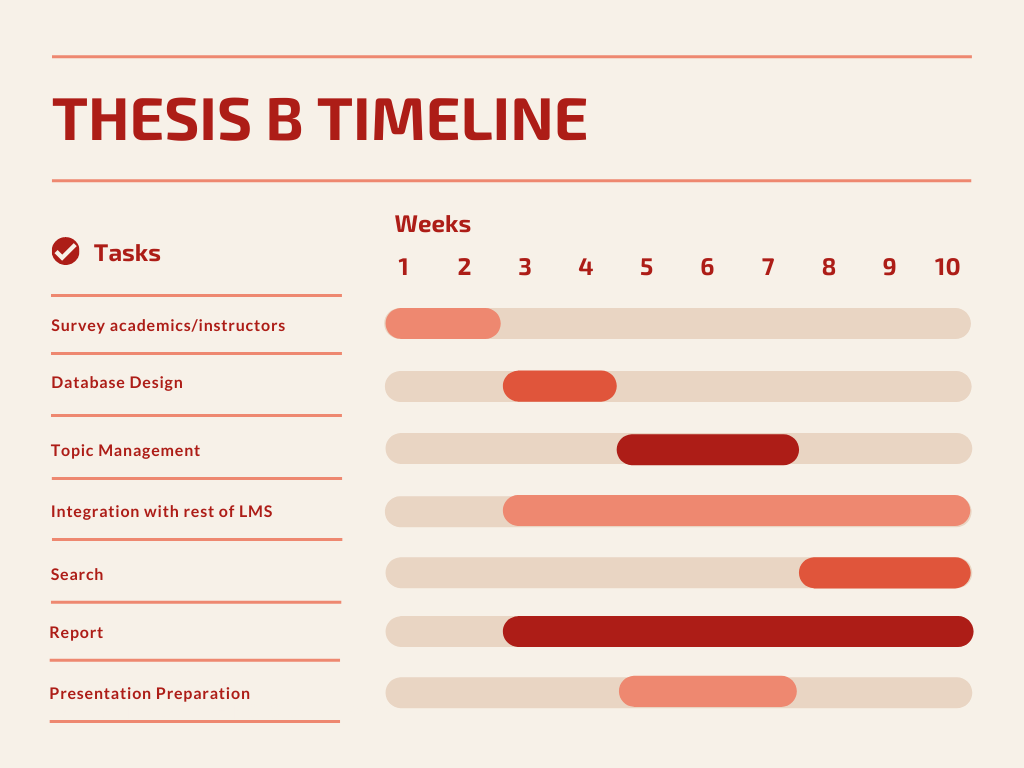
\includegraphics[scale=0.4]{topic-tree-thesis-b}
    \caption{Thesis B Timeline}
\end{figure}

In Thesis B, the focus is to start implementing the topic tree feature, with core features implemented and mostly usable including the graph interface, and a working database design. \\

Database Design will involve designing a schema for the database to store topics and their dependencies. This will most likely involve a graph relationship between topics.\\
Topic Management involves designing the graph interface for adding, removing and managing topics and helping develop a backend for this.\\
Integration with the rest of the system involves using the topic tree to import content into a course, and export content into the topic tree, etc.\\
Search involves searching for content, and is not as important as developing the topic management feature.\\
A graph interface would make it much easier to visualise dependencies between topics, but is not a high priority so the plan is to implement this during Term 2 2021.\\

\begin{figure}[h!]
    \centering
    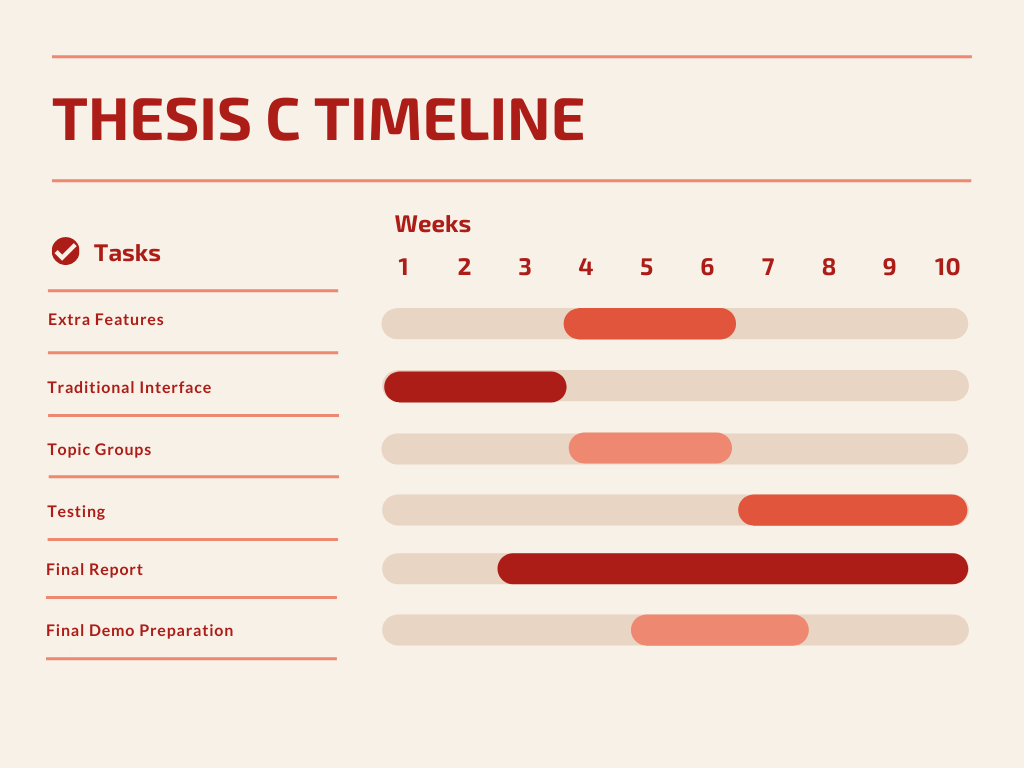
\includegraphics[scale=0.4]{topic-tree-thesis-c}
    \caption{Thesis C Timeline}
\end{figure}

In Thesis C, the main focus is to finalise features, fix any bugs that arise, test the feature and its integration with the rest of the system, implement a traditional interface and allow topics to be grouped with each other.\\

A traditional interface would be easier to use than a graph interface for some users, as it would be more similar to most interfaces used in other software, and would be implemented during Term 3 2021.\\

\newpage
\subsection{Milestones}
Major milestones for the topic tree feature include: \\
\begin{enumerate}
\item Week 6 Term 2 2021 - Implement a database schema for storing topics and their prerequisites, and set up a graph interface for topic management to easily view prerequisites between topics and topic groups.
\item Week 11 Term 2 2021 - Adding and deleting topic prerequisites/dependencies, a search function and proper integration with the rest of the learning management system.
\item Week 6 Term 3 2021 - Traditional interface to improve the user experience of the LMS.
\item Week 11 Term 3 2021 - Final Testing and Analysis of the learning management system.
\end{enumerate}

\subsection{Evaluation}
In order to evaluate how well the feature has met its requirements and achieved its purpose, a criteria will be proposed. \\

This feature will be evaluated in several areas:\\
\textbf{Functional Requirements} \\
The feature must meet all of its functional requirements to ensure that the feature is complete and meets its purpose. Higher priority requirements must be completed before lower priority requirements. Testing tools and data will be used in order to assess its functionality, using tools such as React Testing Library \cite{reactTestingLibrary} and Insomnia Unit Testing \cite{insomniaTesting}.\\

\textbf{Performance} \\
Performance must be high and the feature must be responsive to provide a high quality user experience for both academics and students. Performance will be assessed using tools such as Google Lighthouse \cite{googleLighthouse}. Google Lighthouse uses several metrics to assess performance, as explained previously. \\

\textbf{Accessibility} \\
The topic tree feature will also be assessed on how accessible the interface is. If features such as alt tags, high contrast colours and keyboard navigation are not implemented then not all academics and students will be able to use the topic tree feature. Therefore, tools such as Google Lighthouse will be used to access its accessibility as the tool also includes metrics for measuring accessibility of a website \cite{googleLighthouseAccessibility}. \\

\textbf{Usability} \\
Finally, the feature will be assessed on its usability. This includes whether the topic tree feature is attractive and easy to use. Various students and academics will be surveyed on how easy they found the system to use. The number of errors and time taken to complete a task will also be assessed.\\
